\section{类 Date 的属性}
\hfill\ctli{实验时间}{~2015~年~1~月~12~日}
\subsection*{【实验目的】}
\begin{enumerate}[label={\arabic*、}]
\item 掌握重载的概念
\item 能够进行运算符重载。
\end{enumerate}
\subsection*{【实验环境】}
\MyEnvironment
\subsection*{【实验内容】}
日期类设计

定义Date类,参照实现:
\begin{enumerate}[label={(\arabic*)}]
\item 日期的加、减运算
\item 根据日期计算一年中的第几周星期几、一年中第几天为几月几日、该年是否为闰年
\item 输出日期对象
\end{enumerate}

完成相应应用程序设计
\subsection*{【详细分析】}
首先考虑日期的加减。对于简单的日期对象,加减天数需要正确地识别 0 和 1 的区别,当跨年的时候不可避免地会产生一天的误差。原来我是用一个 \verb|const static int MONTH[2][13]| 来标识月份,并且根据月份进行加减的。但是后来发现这样做对于跨年的处理总是有问题,所以我改用了 \verb|<ctime>| 库中的 \verb|time_t| 和 \verb|struct tm| 来实现我的新 Date 类。这样对于日期的加减就是整数的加减了。

这样产生了另外一个问题,就是 \verb|time_t| 和 \verb|struct tm| 不同步的问题。由于大量的指针操作,我很快被它搞晕了。很快我找到了解决办法,指定 \verb|time_t| 为唯一的标准,而 \verb|struct tm| 则是每次需要时随时转换出来。这样避免了两个表示日期的数据不同步的问题。

这样,计算一年中的第几周、星期几,都可以直接访问 \verb|struct tm| 的属性来获取。一年中的第几天则可以用日期的加减实现。判断闰年则只需要按照规则来就可以了。

需要注意的是,tm\_year 指的是从 1900 年开始的年数,tm\_mon 表示的月份则是从 0 开始的。所以这个类不能够表示 1900 年之前的时间。并且输入输出要做处理。

\subsubsection*{【实验源码】}
{\linespread{1}\lstinputlisting[caption={\tt Date.h}]{exp05/Date.h}}
{\linespread{1}\lstinputlisting[caption={\tt Date.cpp}]{exp05/Date.cpp}}
{\linespread{1}\lstinputlisting[caption={\tt exp01.cpp}]{exp05/exp01.cpp}}
\subsubsection*{【实验结果】}
\begin{figure}[htp]
\centering
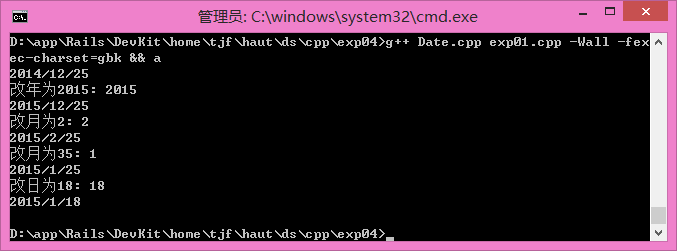
\includegraphics[width=\textwidth]{exp05/exp01.png}
\caption{\label{out05_01}Date 类}
\end{figure}
\subsection*{【实验体会】}

年月日是“历法单位”,不是“时间单位”,历法是人根据天文观测制定的,并不断修正,而“修正”这件事是没有规律的。比如在欧洲大陆,1582年10月5日至10月14日,这10天就是不存在的,调整后的历法就是格里高利历;但是在英国,这个调整一直拖到了一百多年后,直到1752年,这一年的9月3日至13日这11天是不存在的;而在此期间的一百多年里两地的日期一直不相同。

日期时间的处理一直都是比较麻烦的问题。UNIX 的时间戳从 1970~年~1~月~日 开始我觉得是非常合适的办法。使用分开的年月日来表示会产生存储空间的浪费,对于系统来说这是不可以的。自己处理日期时间会不可避免地产生错误,而且由于人为的改历、置闰,程序除非有庞大的数据库支持,才能准确地表示时间。作为简单的面向对象实践,我觉得调用系统库做一个封装,是个非常不错的办法。
